\documentclass[11pt,a4paper]{IEEEtran}

\usepackage[utf8]{inputenc}
\usepackage{amsmath}
\usepackage{amsfonts}
\usepackage{amssymb}
\usepackage{graphicx}
\usepackage{listings}
\usepackage{courier}

\usepackage[style=ieee, backend=biber]{biblatex}
\addbibresource{bibfile.bib}

\author{Tom Eccles}
\title{ELEC2204 Computer Emulation Coursework}

\begin{document}
	\maketitle
	\begin{abstract}
		This document will describe the computer I designed and emulated for this coursework. The design and simulation are timing accurate and model to about the same detail as an implementation written in System Verilog.
	\end{abstract}
	
	\section{Design of the Computer}
	This section will document the design decisions made while designing the computer.
	
			\subsection{Instruction Set Architecture}
			The Instruction Set Architecture outlined here is my own design however it was inspired by the RISC-V Instruction Set by the University of California, Berkeley \cite{riscv}.
			
			To keep the control of the processor as simple as possible, the ISA follows a load-store architecture for main memory access. This results in fewer stages and reduced complexity in the execution of each instruction \cite{bigBook}. It was also decided to make all instructions the same length (one 32-bit word) for simplicity. This has the dissadvantage of (probably) a larger program size in memory \cite{bigBook}. It was not specified that we were to design for an embedded system and so this did not seem important. All data are encoded as Big-Endian. Finally, instructions do not need to be aligned to word boundaries: addresses in memory refer to individual bytes and the first byte of each (4-byte) instruction can be any byte. Individual byte addressing was chosen as a trade-off between flexibility in memory access and maximum possible addressable RAM. 
			
			There are 15 instructions implemented in the processor. Therefore, the op-code could have specified in just 4 bits. However, this would have left very little room for other instructions to be added. I wanted the processor to be extendible so a 5-bit op-code width was chosen. 
			
			Studies in RISC machines shown that it is beneficial to include a large number of registers \cite{smallerBook}. Therefore a 5-bit register index field was chosen: allowing for 32 general purpose registers. This is also the approach taken in RISC-V \cite{riscv} and in MIPS \cite{bigBook}. Choosing these field widths was a trade-off because the more bits which were taken on the op-code and registers, fewer bits are left for the intermediate operand for the \textit{add-immediate} and \textit{sub-immediate} instructions (see upcoming sections). With fewer bits this immediate value looses range. The layout of the instructions can be found in Figure \ref{Fig:instructionBitmap}.
			
			The register at address zero cannot be written to and always contains zero. This allows \textit{add-immediate} to be used to load short immediate value into registers without having to allocate additional memory for the constant and use a load instruction. Furthermore, using this system \textit{add} can be used to copy values between registers and \textit{subtract} can be used to negate values in registers. 
			
			\begin{figure}[!ht]
				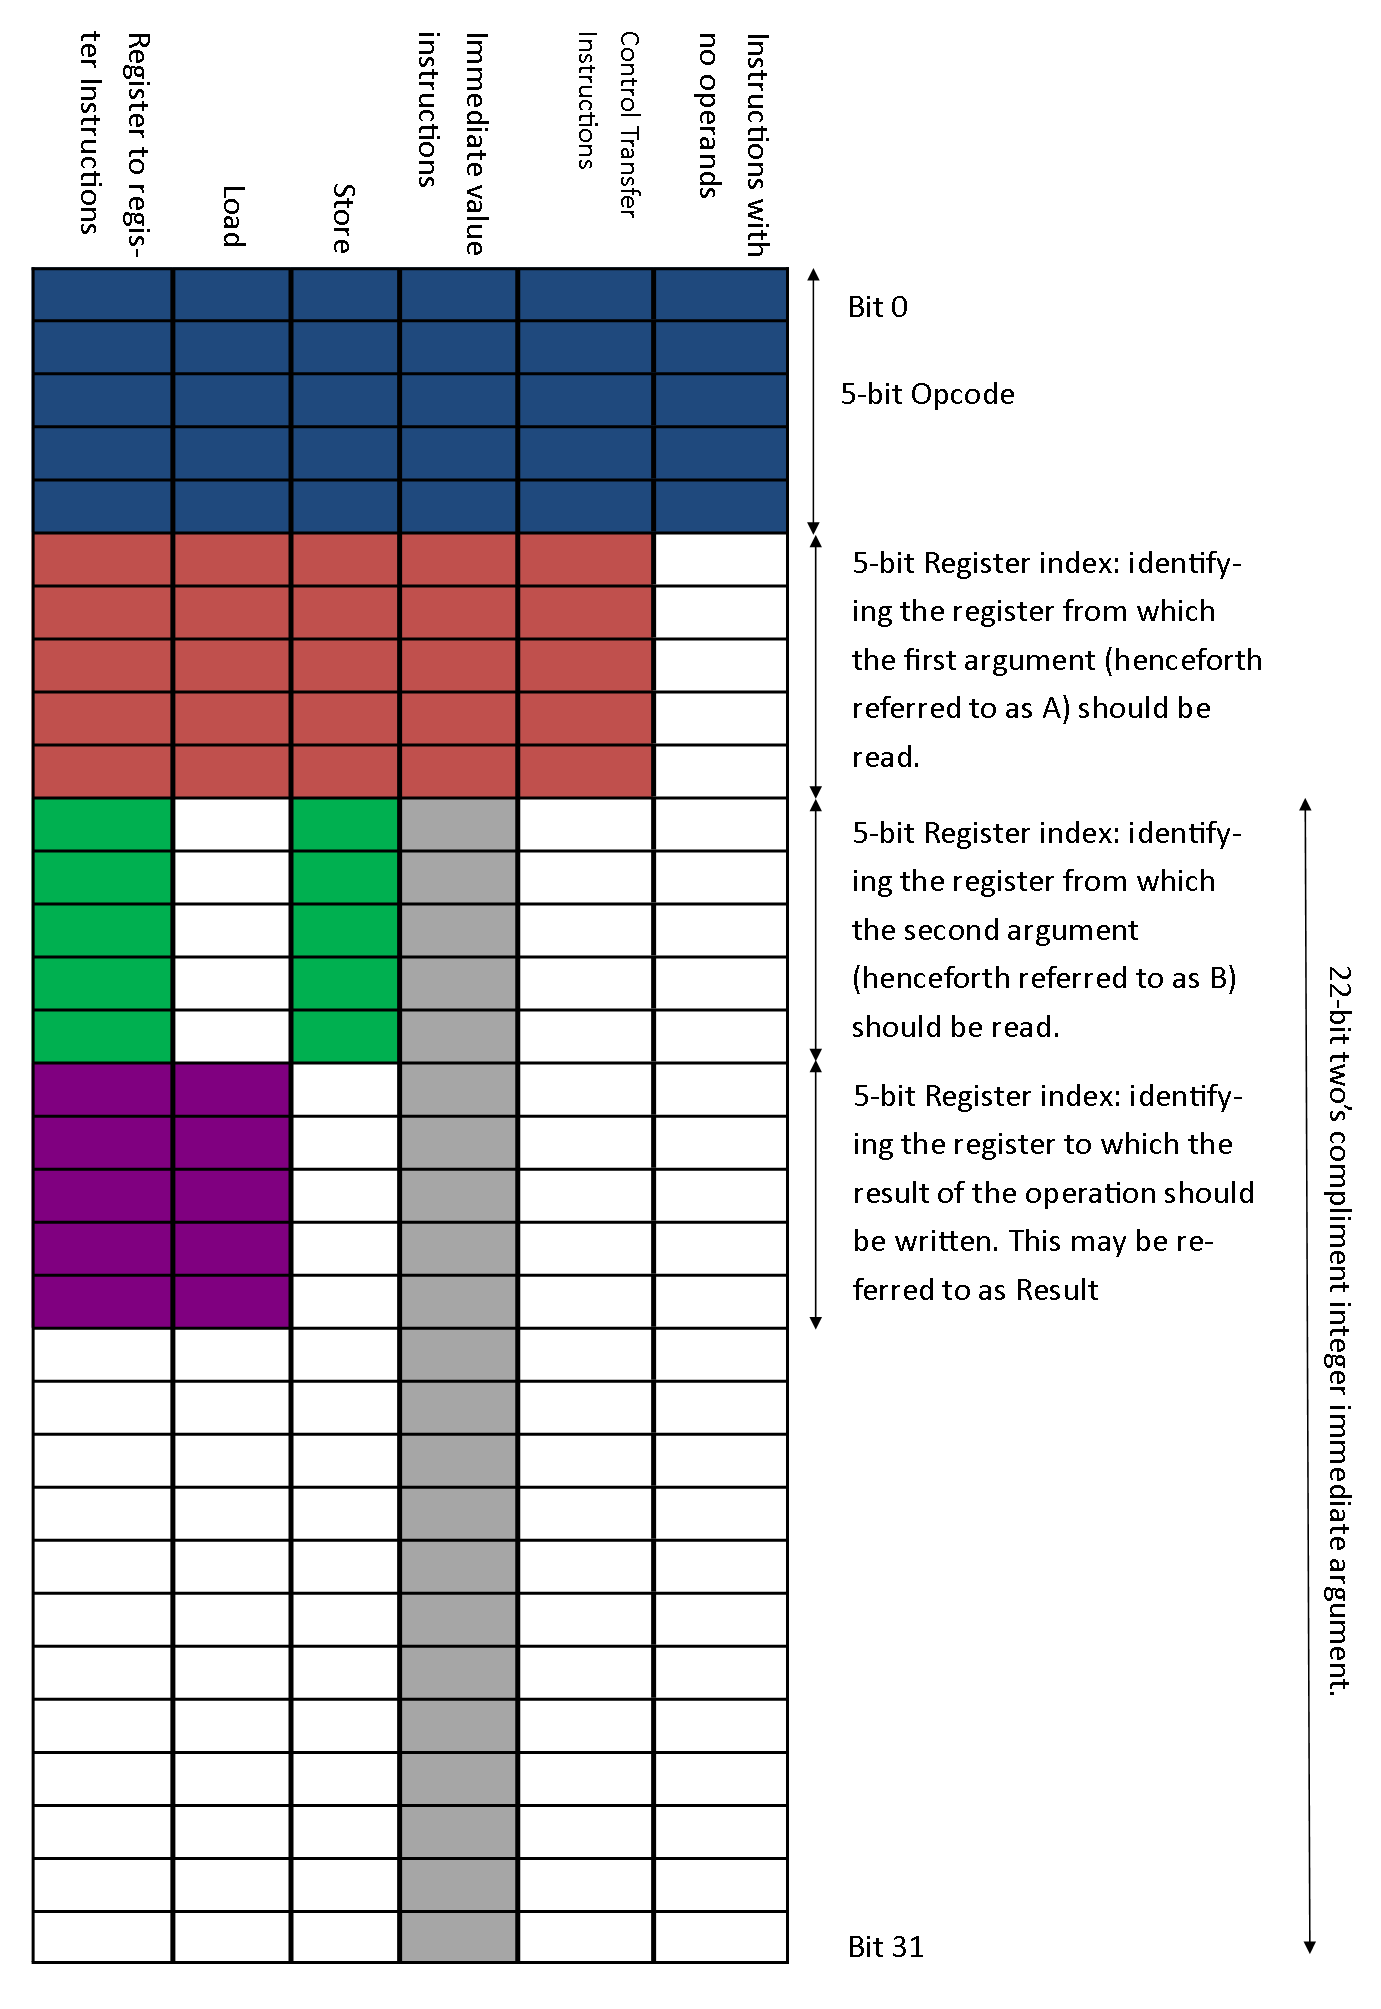
\includegraphics[scale=0.375]{InstructionBitmap.png}
				\caption{Representation of the 5 different instruction types. Cells in the table are colour coded. White cells are bits which are unused in that instruction.}
				\label{Fig:instructionBitmap}
			\end{figure}						
			
			\subsubsection{Register-to-Register operations}
				There are four instructions in this category: \textit{add}, \textit{subtract}, \textit{nand} and \textit{left-shift}. These instructions have three register indices as their operands. If their operation (e.g. $+$ for \textit{add}) is refereed to as OPERATION then their operation can be shown in pseudo-code as follows:
				
				\begin{lstlisting}[language=C]
*Result = *A OPERATION *B;
				\end{lstlisting}
				
				Where * dereferences a register index (similar to pointer dereferencing in C). See Figure \ref{Fig:instructionBitmap} for definitions of A, B and Result.
				
				\textit{nand} Was the only bitwise logic operation included because equivalents for all other boolean logic operations can be constructed from multiple nand operations. \textit{left-shift} Was the only shifting operator included because a right shift would be almost identical code and so it would be easy to add at a later date. The \textit{left-shift} instruction demonstrates that this is possible in the architecture.
				
			\subsubsection{Load Instruction}
				The \textit{load} instruction has two register indices as it's arguments: the register in the A argument position contains the address in memory to be read. The register in the result argument position contains the index of the register to which the word read from memory should be written.
			
			\subsubsection{Store Instruction}
				The \textit{store} instruction also has two register indices as it's arguments: the address in memory to write to and the register who's contents should be written to memory. These arguments are located in the A and B positions, respectively. The positioning of the second argument is different from the second argument in \textit{load} so that all writes to the general purpose registers are addressed by the result argument (as in the register-to-register instructions). Furthermore, the register who's contents should be put on the memory address bus is always indexed by argument A. Keeping these details the same would reduce the complexity of interconnections were this design realised into a real computer because signals of a particular type could only originate from particular outputs of the instruction decoder logic.
			
			\subsubsection{Immediate Value Instructions}
				Two instructions were implemented using this format: \textit{add-immediate} and \textit{sub-immediate}. These instructions use the contents of the register indexed by argument A as the first argument of their operation and the intermediate value as the second argument. It was originally planned for these instructions to also contain a register index to specify where to write the result of the operation. This would have taken 5-bits off the intermediate argument and so would reduce it's range. To avoid this downside, these instructions always behave as though the Result argument identified general purpose register 1 as the location to which to write the result of the operation. Otherwise they behave in the same way as the register-to-register instructions. 
			
			\subsubsection{Control Transfer Instructions}
			The control transfer functions \textit{jump-to-reg}, \textit{jump-if-zero} and \textit{jump-if-positive} each have a single argument in position A. This argument specifies which register contains the absolute memory address to jump to. 
			
			\textit{jump-if-zero} Was included to facilitate jumps if two registers are equal: first the registers would be subtracted and then the processor would jump if the ALU set the zero flag in the subtraction operation. 
			
			\textit{jump-if-positive} Was included to facilitate jumps if one register is larger than another. This would be implemented by first subtracting the registers and then jumping if the positive flag was set in the subtraction operation. 
			
			Originally, relative jump instructions were planned. However due to time considerations these were dropped. Relative jumping would have been implemented by moving the next program counter address calculation into a new stage between Execute and Register Write and using the ALU in the execute stage to calculate the relative address (see Section \ref{sec:InstructionExec} and Section \ref{Sec::Datapath}.) 
				
			\subsubsection{Instructions With No Operands}
				Three instructions were implemented which do not require arguments. These were \textit{nop}, \textit{halt} and \textit{printBuffer}.
				
				The \textit{nop} instruction does nothing. It was included for testing purposes. 
				
				The \textit{halt} instruction ends execution of the program. In the emulated computer this changes a flag to signal that the program has finished. This made it easier to write automated tests for the design. In an actual computer this may drive a signal to turn off the power supply.
				
				The \textit{printBuffer} instruction writes the contents of the video memory to a display. In the simulation this was implemented by writing to the standard output file descriptor after executing a command to clear the console. In a real computer this may signal a display adapter with direct memory access to the video memory to begin outputting the frame in the video buffer to the display interface. For more information on the video memory see Section \ref{sec::splitMemory} on split memory.
				
		\subsection{Split Memory}
			\label{sec::splitMemory}
			The \textit{load} and \textit{store} instructions operate on a single 32-bit address space. However, there are actually two separate instances of the \texttt{RAM} template class: one for general purpose memory and one for video memory. The video memory takes the top 4096 virtual addresses in the total memory size and the rest is general purpose memory. For example, the simulator is configured with 10240 bytes of RAM. This means that addresses 0-6143 refer to the 6kB of general purpose memory. After this, the top 4096 addresses (6143-10239) refer to the video memory. This address translation is performed by the \texttt{RamAddrTran} template class. 
			
			The video memory stores a 64x64 pixel frame buffer where each pixel is stored as a single byte. In the simulation, that byte is displayed as an ASCII character so that the \textit{printBuffer} instruction could be modelled simply.
			
			The computer was originally designed without this split memory functionality and if the \textit{printBuffer} instruction was removed it could be configured without this feature (for example for a system with no display output). To accommodate this, the interface for \texttt{RamAddrTran} is a drop in replacement for \texttt{RAM}. Therefore subsequent sections will just refer to the memory address space from the \textit{load} and \textit{store} instruction's point of view: a single address space.
		
		\subsection{Instruction Execution}
		\label{sec:InstructionExec}
			The execution of an instruction is split into (up to) four stages: Instruction Fetch, Decode, Execute, Register Write. The Register Write stage is skipped for instructions which do not write to the general purpose registers: making these instructions run a little faster. A Datapath diagram illustrating most of this section can be found in Section \ref{Sec::Datapath} (at the end of this report).
			
			\subsubsection{Instruction Fetch}
				In the instruction fetch stage, the instruction addressed by the contents of the Program Counter special purpose register is read from the RAM.
				
			\subsubsection{Decode}
				On the next clock edge, the instruction is read from the RAM's data bus\footnote{As discussed later, it is assumed that all RAM operations finish within one clock cycle. On a real machine this would not be true but I did not have time to implement the cache model extension task.} and decoded. With the instruction format shown in Figure \ref{Fig:instructionBitmap}, the decoding is very simple. Outputs A, B and Result only need to be wired directly to the correct bits of the input. The immediate value requires sign-extension to be a 32-bit value appropriate for input to the ALU. 
				
				The opcode, result and immediate outputs of the decoder are saved to special purpose registers so that they will be available in the next clock cycle. Arguments A and B are sent to the two read channels of the general purpose register file for reading. 
				
				Also in the decode stage, the ALU is used to calculate the program counter plus one word length and save this into the \texttt{PCplus4} special purpose register. This is used in the execute stage to determine the next value of the program counter. 
			
			\subsubsection{Execute}
				On the next clock edge, the newly read data from the register file are used as follows depending upon the instruction type:

				\begin{itemize}
					\item For register-to-register instructions these data are used as the arguments to the ALU.
					\item For the \textit{load} instruction, the RAM control signal is set to read and output A of the register file is used as the address for the RAM.
					\item For the \textit{store} instruction, the ram control signal is set to write, output A of the register file is used as the address for the RAM and output B of the register file is used as the data to be written to the RAM.
					\item For immediate value instructions, the A output of the register file is used as the first argument to the ALU and the Immediate register output is the second argument to the ALU. 
					\item For control transfer instructions, the A output of the register file is used as an input to the relevant multiplexer to ultimately choose the new value for the program counter. For the conditional jump operations, the output of the relevant ALU flag register is used to control the multiplexer between this value and the value of \texttt{PCplus4}. The ALU flag registers will have not yet clocked in the new values from the ALU from this cycle and so will output their values from the previous instruction. 
					\item \textit{halt} And \textit{nop} do nothing here. In a hardware implementation, \textit{halt} might change a control signal to the power supply. 
					\item In simulation, \textit{printBuffer} writes the contents of the video memory to the standard output file descriptor. As already discussed, this would be different in a hardware implementation.
				\end{itemize}								
				 
			\subsubsection{Register Write}
				This cycle is skipped for instructions which do not write to the register file. The control signal for the register file is set to write. For immediate value instructions, the write select input is set to 1, otherwise it is the output of the register in which the result argument of the instructions was stored. For a load instruction the write data input of the register file is set to the data just read from RAM. Otherwise it is the output of the register to which was saved the result of the ALU in the previous stage.			
			
	\section{Design of the Emulator}
                The emulator is designed to conduct all of the combinational logic first and then write to registers at the end of the processing for each clock cycle. This was inspired by the system of blocking and non-blocking assignments in Verilog.

		\subsection{Combinational Logic}
			To be sure that the emulator was accurate to the design, it was important that emulated combinational logic worked like real combinational logic: with no memory. It had already been decided to implement each module in the computer as it's own class because this would make the interfaces within the computer clearer: making the code more readable and making the code easier to expand upon in the future. To fit this design, combinational logic is implemented in the get/set methods of the classes. When outputs of that module are read (using public get methods), a check is performed to ensure that the value being read is a defined logic level with a sensible value. This provides some testing as any code is executed and by setting outputs to be considered undefined after each clock tick, it prevents classes containing only combinational logic from remembering their values as though they contained registers.
			
			\subsubsection{Signal}
				It did not seem sensible to implement the previously mentioned functionality separately in every class so it is all included in the \textit{Signal} template class. This can be found in \texttt{emulator/Signal.h}. 
				
				\texttt{Signal} objects are constructed with the undefined flag set. While this flag is set, Signal will print an error message and abort the simulation if it's data are read. When it is assigned a value the undefined flag is removed until the \texttt{undefine} method is called.
				
				For \texttt{Signal} to correctly model combinational logic, the \texttt{undefine} method should be called at each clock tick event to ensure that the value on the output is not remembered into the new clock cycle.
			
			\subsubsection{Mux}
				In a similar manner to \texttt{Signal}, \texttt{Mux} (\texttt{emulator/mux.h}) needed to be as general as possible so that multiplexing functionality would only need to be implemented once. 
				
				In order to allow \texttt{Mux} to multiplex between any number of inputs, the input values are stored in a \texttt{std::unordered\_map} allowing them to be retrieved by sending the correct control signal (the key to the hash table.)
				
				\texttt{Mux} also contains an \texttt{undefine} method for the same purpose as the one in \texttt{Signal}.
		
		\subsection{Sequential Logic}
			All of the sequential logic is implemented using the \texttt{Register} template class.
			\subsubsection{Register}
				\texttt{Register} contains two \texttt{Signal} objects: the current value at the output of the Register and what the output will change to at the next clock edge. \texttt{Signal} objects were used so as to provide the error checking it implements. This ensures that the output of a \texttt{Register} is not read while it contains an undefined value. It is implemented in \texttt{emulator/Register.h}.	
				
				\texttt{Register} does not behave like a standard flip-flop. The output is not always set to the input on a clock edge. Instead, the Register will retain it's current value until explicitly written to. Figure \ref{fig::reg} shows a better representation of this functionality. The \textit{Write Enable} signal in the figure is not included explicitly in \texttt{Register}. Instead it is implicit in the \texttt{changeDriveSignal} method.
				
				\begin{figure}[!h]
					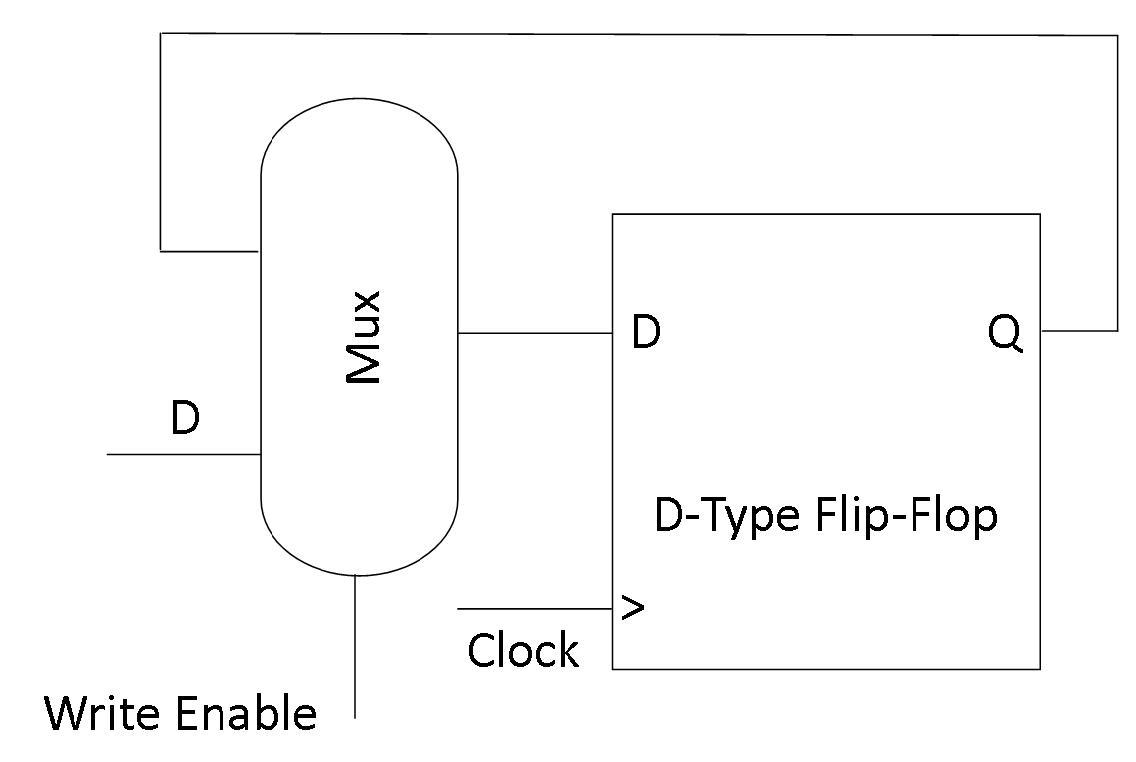
\includegraphics[scale=0.35]{Register.png}
					\caption{The operation of the \texttt{Register} template class}
					\label{fig::reg}
				\end{figure}			
			
			\subsubsection{RegisterFile}
				\texttt{emulator/RegisterFile.h} Is a template class used in the computer emulator to represent the general purpose registers. \texttt{RegisterFile} was deliberately over generalised so that it would not need to be re-written if changes were made to the design of the processor. 
				
				\texttt{RegisterFile} contains one write channel and two read channels. This was the minimum required to satisfy the design shown in Section \ref{Sec::Datapath}. 
				
				All of the inputs and outputs are stored using \texttt{Signal} objects. This provides a way of keeping track of which inputs were set during that clock cycle. The general purpose registers themselves are constructed using an array of \texttt{Register} objects so that they can be easily indexed with the register index instruction operands.

			\subsubsection{RAM}
				As a cache model was considered optional extension work, the speed of RAM access was not considered in the design. The RAM was modelled as a very large number of single byte registers. In a real computer system, RAM is significantly slower than registers. The processor would have to stall execution while waiting for RAM accesses to complete. 
	
				The \texttt{RAM} template class in the simulator is similar to \texttt{RegisterFile} except with a bidirectional data bus and the ability to pre-load the memory with some data before the emulator starts. This was important for the RAM because the processor will begin executing the instruction at address 0 in the RAM. Therefore the program to be executed and any data it required needed to be loaded into the RAM first. 
	
	\section{Testing}
	Every module is tested individually using the test programs contained in the \texttt{test} directory. 
	
	The computer is also tested as a whole using several assembly language programs in \texttt{test/cpuTest.cpp} and \texttt{test/cpuDemo.cpp}. The programs are written symbolically using \texttt{Instruction } (\texttt{assembler/Instruction.cpp}) objects. \texttt{Instruction} can produce a correct machine code word for that assembly instruction. A \texttt{std::vector} of these assembled words is preloaded into the RAM before the processor begins operation.
	
	\texttt{RAM} also provides the \texttt{debugRead} method. \texttt{debugRead} reads straight from the \texttt{Register} array without modelling any real world hardware. This allows the tests for the whole computer to check that the correct value was written to the correct address in RAM at the end of the test program. 
	
	Signals can be captured to standard error (usually connected to the console which executed the tests) by defining the \texttt{DEBUG\_SIGNAL} preprocessor macro. Non-fatal warnings and information about test passes can be captured to standard error by defining \texttt{DEBUG}. Both of these macros are defined when building using the makefile provided with the source code. The printing functions can be found in \texttt{emulator/debug.h} and \texttt{emulator/debug.cpp}. 
	
	The \texttt{cpuDemo} test program (\texttt{tests/cpuDemo.cpp}) was written to show off the capabilities of the video memory. It animates a "Hello World!" message travelling across the screen.
	%\pagebreak
	\printbibliography	
	%\pagebreak
	\section{Appendix - Datapath Diagram}
	\label{Sec::Datapath}
	In order to make this diagram easier to read, some modules of the processor are drawn twice in different stages. This does not indicate different instances of these modules. For example, the ALU pictured in the Decode stage is the same ALU used in the Execute stage. See \texttt{doc/Datapath.png} for a larger version of the diagram.

	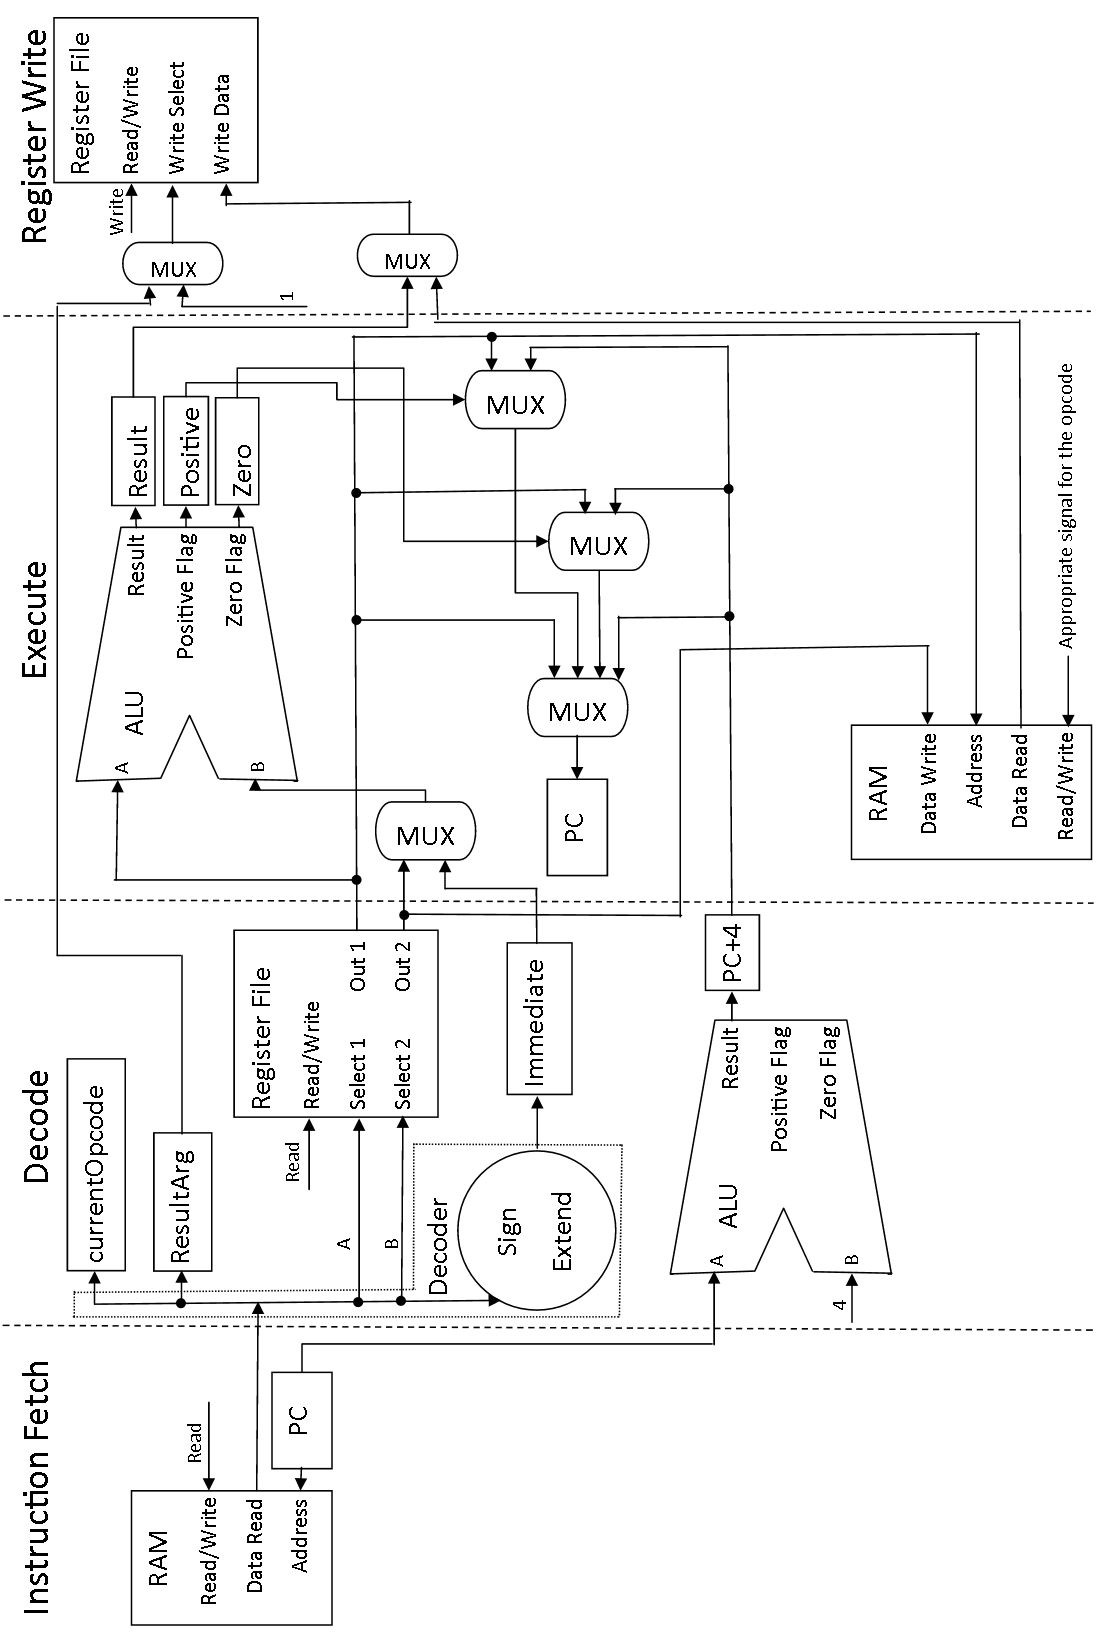
\includegraphics[scale=0.45]{Datapath.png}
	

\end{document}
